\documentclass[preprint,12pt]{elsarticle}
\usepackage{fontspec}
\setmainfont{TeX Gyre Termes}
\usepackage{amsmath,amssymb,booktabs,longtable,array,graphicx,adjustbox,placeins,calc,caption,float,xurl}
\usepackage[unicode,colorlinks=true,allcolors=blue]{hyperref}
\providecommand{\tightlist}{\setlength{\itemsep}{0pt}\setlength{\parskip}{0pt}}
\newcounter{none}
\providecommand{\pandocbounded}[1]{\begin{adjustbox}{max width=\linewidth,max totalheight=.65\textheight,keepaspectratio}#1\end{adjustbox}}
\setlength{\emergencystretch}{3em}
\setlength{\intextsep}{10pt plus 2pt minus 2pt}
\makeatletter
\def\ps@pprintTitle{\let\@oddhead\@empty\let\@evenhead\@empty\def\@oddfoot{\footnotesize\itshape Working manuscript, v23\hfill\today}\let\@evenfoot\@oddfoot}
\makeatother
\begin{document}
\begin{frontmatter}
\title{Preserving physical information in transferable wind-power event measurements}
\author[aff1,aff2]{Peiyan Gong}
\ead{202483300332@nuist.edu.cn}
\author[aff1,aff2]{Chaoxia Yuan\corref{cor1}}
\ead{chaoxia.yuan@nuist.edu.cn}
\cortext[cor1]{Corresponding author.}
\address[aff1]{State Key Laboratory of Climate System Prediction and Risk Management/Key Laboratory of Meteorological Disaster, Ministry of Education/Collaborative Innovation Center on Forecast and Evaluation of Meteorological Disasters, Nanjing University of Information Science and Technology, Nanjing 210044, China}
\address[aff2]{Jiangsu Key Laboratory of Intelligent Weather Forecasting and Applications Based on Big Data/School of Artificial Intelligence, Nanjing University of Information Science and Technology, Nanjing 210044, China}
\begin{abstract}
Wind-power event measurements must preserve the distinctions needed for physical interpretation and operational decisions. We introduce a four-layer framework linking detection, matching, representation and evaluation. Across seven primary wind-farm archives comprising 333 turbines, plus a seven-turbine instrumented French archive, 17 detector configurations establish a broad comparison of event measurements. Ordered trajectories provide a transferable structural reference, with median adjusted Rand index (ARI), a chance-corrected measure of partition agreement, of 0.714--0.817 across the primary archives. A signed-domain Gramian angular field maps a trajectory and its sign reversal to the same image. Preserving a polarity coordinate within a six-dimensional representation restores directional information: calibration against independent light detection and ranging (LiDAR) observations raises the area under the receiver operating characteristic curve from 0.494/0.477 to 0.890/0.905 at two instruments. In an exploratory British observed-price replay, large-ramp periods contribute 54--71\% of persistence gross debits, and historical event information reduces two-hour debit exposure by 4.48\% within a matched forecasting model. Together, the experiments establish a method for selecting event descriptions through structural survival, independent physical tracking and decision-specific value.

\end{abstract}
\end{frontmatter}
\FloatBarrier
\section{Introduction}\label{introduction}

Wind-power forecasting turns atmospheric variability into information for reserve scheduling, trading and flexible operation. Physical, statistical and learning-based methods have improved this conversion, while probabilistic forecasting has made forecast uncertainty part of the operational question \citep{foley2012, pinson2013, hong2016}. Dynamic events provide an intermediate description between a continuous trajectory and an action: they locate when production changes, characterize how it changes and identify the time over which a response may be useful.

The event itself is a measurement choice. Ramp research has defined changes through amplitude, duration, timing and local trend \citep{gallego2015, zhang2025rampreview}. Swinging Door and optimized segmentation methods construct interval boundaries, while threshold, historical-tail and ordinal approaches emphasize different aspects of variability \citep{florita2013, cui2015, ramp_piecewise2023, var2024, ordinal2023}. A large excursion that returns to its initial level illustrates the distinction: it has a small net change and a substantial internal dynamic structure. The scientific question is which of these structures remains recognizable when the measurement protocol changes.

Modern forecasting makes this question more consequential. Event grouping, stochastic scenarios, attention, transfer learning and multiscale models offer increasingly expressive representations of production changes \citep{trend2023, cui2015stochastic, multitask2024, rampattention2024, temporal2024, transfer2023}. Recent event-aware and probabilistic wind-power models connect architectural improvements to operational prediction \citep{apenergy124068, apenergy123487}. Time-series representations also range from ordered coordinates to image encodings and learned temporal features \citep{fawaz2019, wang2015gaf, wu2023timesnet, zhou2025kanad}. Their comparison therefore requires a shared definition of the process being represented, as well as a test of the information that the representation preserves.

Independent atmospheric measurements supply that test. Weather regimes, coupled wind-farm dynamics and spatial inflow variations all influence production trajectories \citep{regimes2015, coupled2024, apenergy125135}. Large-farm evaluations and numerical-weather-prediction studies demonstrate the importance of weather-model configuration, resolution and timing \citep{jin2024, bianco2025, nwpattention2023}. Event structure can consequently be evaluated in two complementary directions: weather information can predict production changes, and observed production structure can support probabilistic identification of the associated wind process. These directions connect event measurement to physically interpretable forecasting.

Here we organize wind-power event evaluation into four layers: detection, matching, representation and evaluation--decision (Fig.~\ref{fig:main1}). Detection defines intervals; matching establishes correspondence; representation and clustering describe their structure; evaluation tests their physical and operational use. Three criteria connect these layers. Structural survival measures partition agreement among corresponding events; coverage is the fraction of eligible events represented in a match, reported separately for each side. External-process tracking tests whether the representation identifies independently measured wind dynamics. Forecast-to-cost validation evaluates available information under the timing and prices of a decision. Chinese and European archives share the same physical-time interface, and a reserved later period tests frozen representations across time.

\begin{figure}[H]
\centering
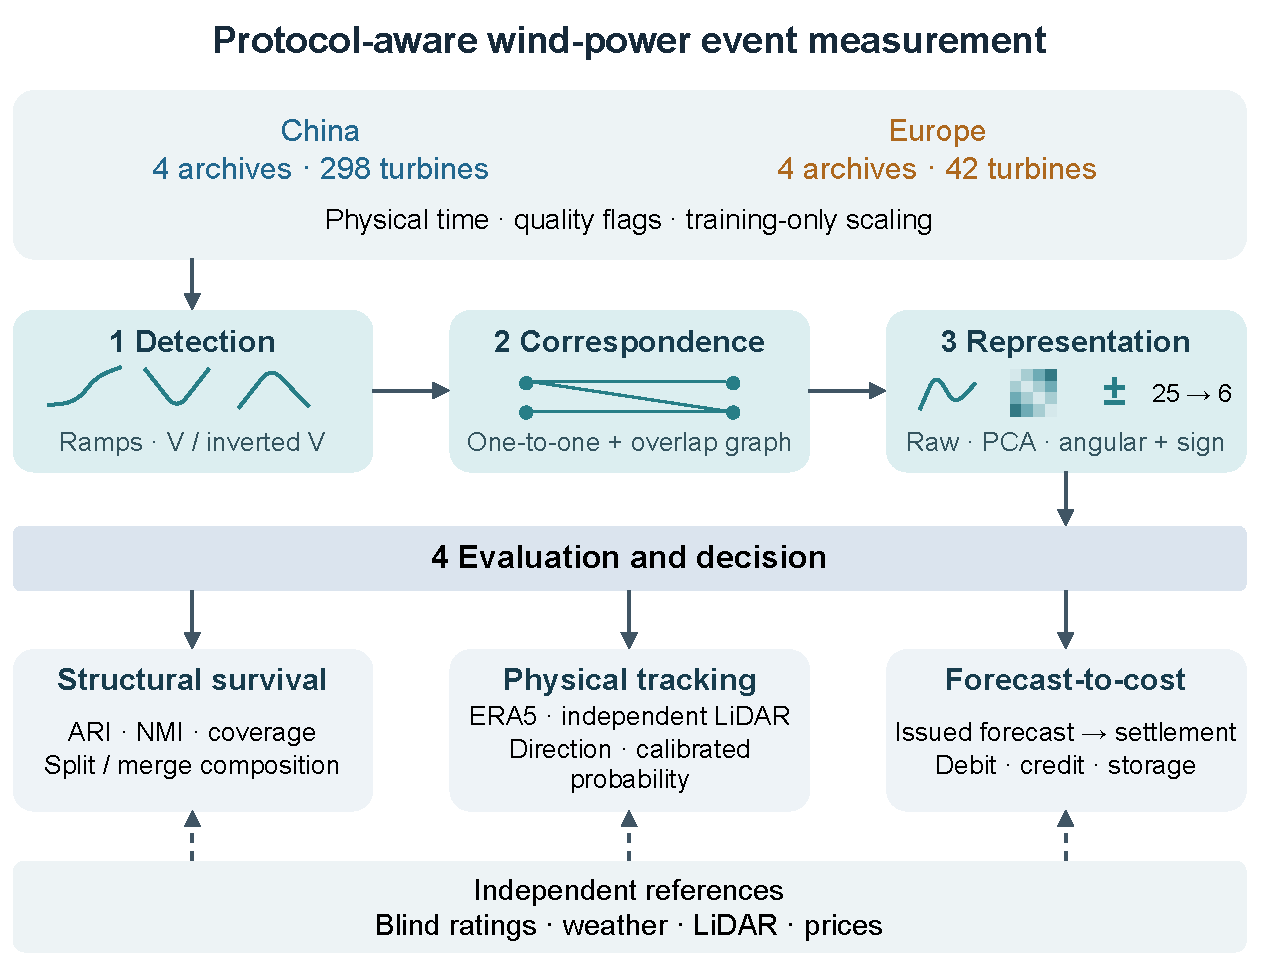
\includegraphics[width=\linewidth]{fig01_workflow.pdf}
\caption{Four layers connect eight wind-farm archives (340 turbines) to three validation criteria. Detection defines ramp and compound intervals; correspondence uses one-to-one matches and split/merge overlap graphs; representations retain trajectory or angular information. Structural survival, external-process tracking and forecast-to-cost tests evaluate progressively different uses. Miniature trajectories, overlap links and the angular field are schematic. China and Europe identify data regions; panel fills distinguish measurement from evaluation. Dashed arrows supply independent reference evidence. Hill 2021 and 2026 are additional periods from the same farm.}
\label{fig:main1}
\end{figure}

We establish a task-aware approach to event measurement. Matched-event comparisons identify trajectory structures that persist across detection protocols, and independent human assessments test whether the intervals locate recognizable changes. We then isolate a global-sign ambiguity in signed-domain angular encoding and protect polarity within a fixed-dimensional representation. Regional weather and independent LiDAR observations test the physical information restored by this design. Finally, an observed-price forecasting track connects available historical event information to settlement exposure. The central proposition is that structural stability and physical discrimination are complementary design criteria, with decision value evaluated when the information becomes available.

\FloatBarrier
\section{Results}\label{results}

\subsection{A common physical-time interface supports transferable event structure}\label{a-common-physical-time-interface-supports-transferable-event-structure}

The harmonized catalogue contains 4,542,258 candidate intervals and 3,226,925 complete 25-coordinate shapes from seven archives and 333 turbines. Basic detector intervals and composite V-shaped or inverted-V episodes form separate event levels. Seventeen detector configurations share a 30-min grid, physical lags of 60, 120 and 240 min, a 24-h historical window and two hours of context on each side. Fig.~\ref{fig:main2} applies these rules to the same measured production trajectory, making protocol-dependent event boundaries visible before the aggregate comparison.

\begin{figure}[H]
\centering
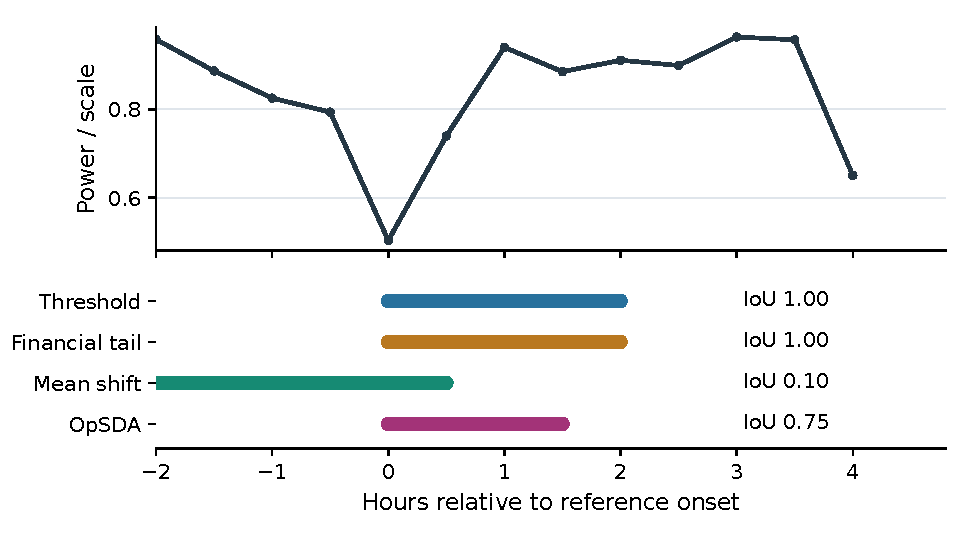
\includegraphics[width=\linewidth]{fig02_detection.pdf}
\caption{The same observed trajectory yields different event boundaries. The lower tracks show the four detector intervals on the same physical-time axis; threshold and financial-tail boundaries coincide in this example. IoU is measured against the threshold reference. Track labels replace an overlapping legend.}
\label{fig:main2}
\end{figure}

Pizhou and Greece each supply 9,925 training events under a matched sampling budget. Six representations, three clustering algorithms, three cluster counts and three seeds yield 324 fitted source models and 648 source--target evaluations. The primary analysis fixes K-means at k=4; k=2 and k=6 test coarser and finer partitions. On the configuration pairs shared by all six primary representations and all three seeds, raw25 median adjusted Rand index (ARI) ranges from 0.714 to 0.817 across the seven archives. ARI measures agreement between cluster partitions after correcting for random agreement: 1 denotes identical partitions up to relabelling, 0 the chance expectation, and negative values less agreement than expected by chance. A supported configuration pair contains at least 100 matched event pairs; a primary informative pair additionally has nonconstant partitions in both protocols. Greece provides 66 such supported configuration pairs and median ARI 0.817; the reserved Hill 2021 period provides 112 and ARI 0.711. An event pair is one matched interval from each protocol, whereas a configuration pair is the pair of detector settings being compared.

{\def\LTcaptype{none} % do not increment counter
\begin{longtable}[]{@{}
  >{\raggedright\arraybackslash}p{(\linewidth - 8\tabcolsep) * \real{0.2000}}
  >{\raggedleft\arraybackslash}p{(\linewidth - 8\tabcolsep) * \real{0.2000}}
  >{\raggedleft\arraybackslash}p{(\linewidth - 8\tabcolsep) * \real{0.2000}}
  >{\raggedleft\arraybackslash}p{(\linewidth - 8\tabcolsep) * \real{0.2000}}
  >{\raggedleft\arraybackslash}p{(\linewidth - 8\tabcolsep) * \real{0.2000}}@{}}
\toprule\noalign{}
\begin{minipage}[b]{\linewidth}\raggedright
Archive
\end{minipage} & \begin{minipage}[b]{\linewidth}\raggedleft
Turbines
\end{minipage} & \begin{minipage}[b]{\linewidth}\raggedleft
Candidates
\end{minipage} & \begin{minipage}[b]{\linewidth}\raggedleft
Complete shapes
\end{minipage} & \begin{minipage}[b]{\linewidth}\raggedleft
Validation + test matches
\end{minipage} \\
\midrule\noalign{}
\endhead
\bottomrule\noalign{}
\endlastfoot
Pizhou & 33 & 880,613 & 606,140 & 611,159 \\
Suining & 14 & 287,061 & 227,472 & 243,765 \\
Yandun & 117 & 669,958 & 539,542 & 1,078,205 \\
La Haute Borne & 4 & 83,622 & 75,402 & 74,258 \\
Hill of Towie 2020 & 21 & 518,078 & 468,272 & 478,528 \\
Greece & 10 & 64,286 & 54,249 & 40,164 \\
SDWPF & 134 & 2,038,640 & 1,255,848 & 2,516,079 \\
Hill of Towie 2021 & 21 & 182,660 & 168,236 & 449,388 \\
\end{longtable}
}

Match counts in this catalogue table include both event hierarchies and the validation and test periods. The structural comparison below uses basic-interval test events. Supported pairs are detector-configuration pairs with at least 100 matched events and informative partitions common to the representations. Coverage is the mean left/right catalogue fraction across all configuration comparisons, reported separately from agreement on the supported subset.

{\def\LTcaptype{none} % do not increment counter
\begin{longtable}[]{@{}
  >{\raggedright\arraybackslash}p{(\linewidth - 8\tabcolsep) * \real{0.2000}}
  >{\raggedleft\arraybackslash}p{(\linewidth - 8\tabcolsep) * \real{0.2000}}
  >{\raggedleft\arraybackslash}p{(\linewidth - 8\tabcolsep) * \real{0.2000}}
  >{\raggedleft\arraybackslash}p{(\linewidth - 8\tabcolsep) * \real{0.2000}}
  >{\raggedleft\arraybackslash}p{(\linewidth - 8\tabcolsep) * \real{0.2000}}@{}}
\toprule\noalign{}
\begin{minipage}[b]{\linewidth}\raggedright
Archive
\end{minipage} & \begin{minipage}[b]{\linewidth}\raggedleft
Supported pairs
\end{minipage} & \begin{minipage}[b]{\linewidth}\raggedleft
Raw25 ARI
\end{minipage} & \begin{minipage}[b]{\linewidth}\raggedleft
Left coverage
\end{minipage} & \begin{minipage}[b]{\linewidth}\raggedleft
Right coverage
\end{minipage} \\
\midrule\noalign{}
\endhead
\bottomrule\noalign{}
\endlastfoot
Pizhou & 105 & 0.747 & 34.5\% & 30.9\% \\
Suining & 98 & 0.724 & 34.5\% & 32.5\% \\
Yandun & 119 & 0.714 & 34.6\% & 35.5\% \\
La Haute Borne & 89 & 0.785 & 32.2\% & 32.3\% \\
Hill of Towie 2020 & 104 & 0.717 & 34.8\% & 32.8\% \\
Greece & 66 & 0.817 & 31.2\% & 29.7\% \\
SDWPF & 119 & 0.745 & 33.5\% & 31.1\% \\
Hill of Towie 2021 & 112 & 0.711 & 33.4\% & 33.2\% \\
\end{longtable}
}

The 2021 evaluation adds a period from the same 21 Hill of Towie turbines. Its 168,236 complete shapes and 367,102 basic-interval test matches extend the temporal test while retaining the original training transformations. Coverage is recorded separately for each side of every match, so the comparison has an explicit population as well as an agreement score.

A metric sensitivity reuses the frozen Pizhou K-means models at k=4 and seed 41. Raw25 ranks above ordinary angular principal component analysis (PCA) and protected-polarity angular PCA at all seven archives and the reserved period under adjusted mutual information (AMI), the Fowlkes--Mallows index and variation of information (VI), as well as ARI and normalized mutual information (NMI). The single-seed comparison uses the same supported event pairs for all three representations. Agreement across these metrics strengthens the interpretation of raw25 as a stable structural reference, while the following experiments evaluate the distinct physical information retained by angular representations.

Raw--PCA6 is a compression control derived from the same 25-point trajectory (Fig.~\ref{fig:main3}). It retains 93.4\% of standardized Pizhou training variance. Across the three seeds, the ARI between its Pizhou test partition and the corresponding raw25 partition is 0.985--0.998. Cross-protocol site medians differ by −0.0022 to 0.0027 across the seven primary archives (Fig.~\ref{fig:main4}), with full-precision configuration differences archived alongside the summaries. The retained low-dimensional trajectory structure explains the close values.

\begin{figure}[H]
\centering
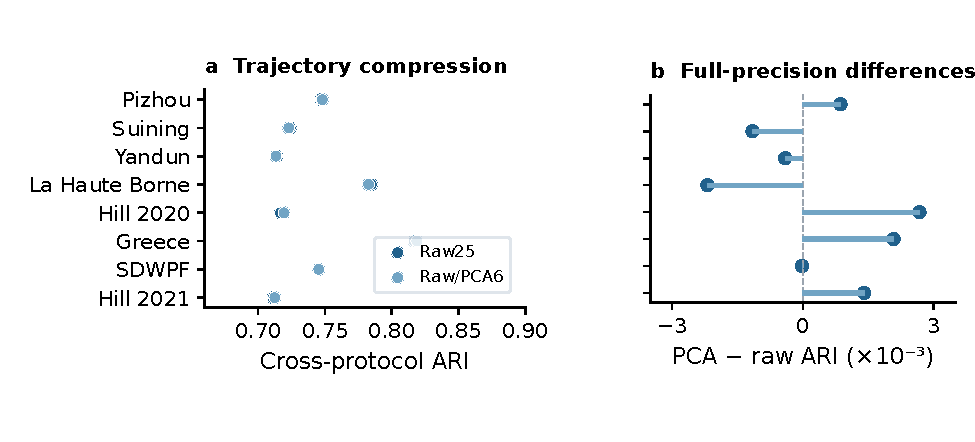
\includegraphics[width=\linewidth]{fig03_compression.pdf}
\caption{Raw/PCA6 provides a compression control for the same 25-point trajectory. Panel a shows current common-support v18 results; panel b resolves differences hidden by two-decimal rounding. PCA retains 93.4\% of standardized training variance. The separate event-label partition comparison is reported in the accompanying data; it differs from cross-protocol ARI.}
\label{fig:main3}
\end{figure}

The primary k=4 comparison resolves four empirical groups rather than four prescribed physical classes. Cluster-count sensitivity is reported explicitly in Supplementary Table S57. In the common-support Pizhou comparison, raw25 median ARI is 0.930, 0.747 and 0.653 at k=2, 4 and 6, respectively; the corresponding ordinary GAF/PCA values are 0.147, 0.227 and 0.284. Raw25 remains above angular PCA at all three cluster counts in Pizhou, Greece and Hill 2021. At k=6, statistics9 reaches ARI 0.835 in Greece and 0.651 in Hill 2021, exceeding raw25 at 0.735 and 0.587. These results identify a resolution-dependent comparison: coarse trajectory groupings transfer strongly, while finer scalar partitions can preserve additional distinctions. The complete six-representation k=2/6 contrasts concern these three evaluation populations; raw25-only k=2/6 transfer is also reported for the other archives. The corresponding primary comparison is shown in Fig.~\ref{fig:main4}.

\begin{figure}[H]
\centering
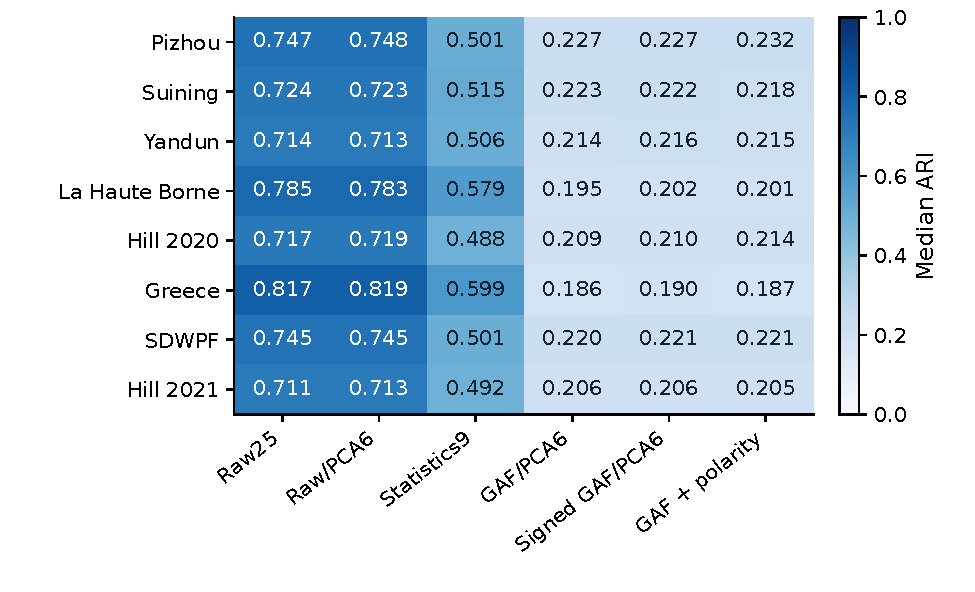
\includegraphics[width=\linewidth]{fig04_structure.pdf}
\caption{Structural survival across seven archives and the Hill 2021 temporal holdout. Darker blue represents higher ARI; label contrast follows cell luminance. Each cell is the median over common detector-configuration pairs after the median over three training seeds. Raw/PCA6 and the angular variants are related ablations, whose differences are resolved in Fig.~\ref{fig:main3} and the full-precision data.}
\label{fig:main4}
\end{figure}

\subsection{Protocol perturbations identify a stable core and complementary geometry}\label{protocol-perturbations-identify-a-stable-core-and-complementary-geometry}

An overlap graph extends correspondence to event splitting and merging. At IoU ≥ 0.5, 6.6--9.5\% of primitive-event overlap components contain more than one event on at least one side. Including primitive and composite V/inverted-V intervals raises this share to 19.8--36.7\% across the seven archives and Hill 2021. This quantifies the additional correspondence revealed when a single compound change is represented as several detector intervals. One-to-one pairing supports event-level partition agreement, whereas the overlap graph preserves the split/merge composition of shared episodes (Supplementary Table S58 and Fig. S1).

Changing an amplitude threshold changes the event population and its boundaries. Across all seven archives, thresholds of 0.10, 0.15, 0.25 and 0.30 were compared with the 0.20 reference using frozen amplitude scales and prototypes. Financial-tail probabilities of 0.01, 0.025 and 0.10 were similarly compared with the 0.05 reference. Crossing these seven perturbations with three lags (60, 120 and 240 min) and seven sites gives 147 site--parameter--configuration comparisons, each carrying one-to-one event matches and separate left/right coverage. These tests identify which measured structures survive a controlled change to the detector; the sampling examples in Fig.~\ref{fig:main5} show the same physical-time principle under changes to the observation grid.

Sampling provides a second physical perturbation. The same-context Greek 30-versus-60-min comparison gives a median ARI of 0.942, with median minimum-side coverage of 0.484. Greek 10-versus-30-min values are 0.866 and 0.551. At Yandun, 15-versus-30-min values are 0.761 and 0.708. The added 30-versus-60-min comparisons give median ARI 0.857 for La Haute Borne and 0.794 for Hill of Towie, with median matched-side coverage 0.396 and 0.412 among configurations with at least one match. Fig.~\ref{fig:main5} displays the full detector-configuration distributions behind these summaries. Agreement and coverage have distinct meanings: a retained structure can remain recognizable among matched events while the observation grid changes which intervals can be compared.

\begin{figure}[H]
\centering
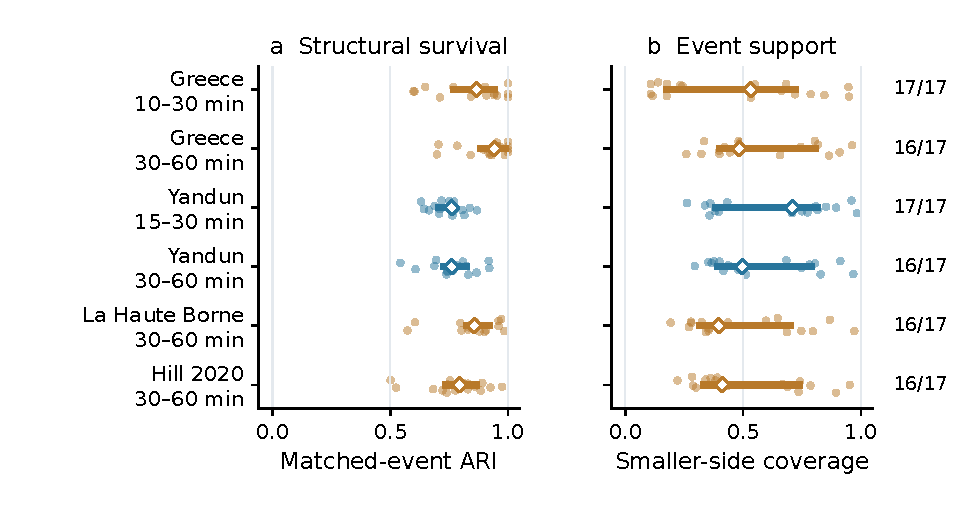
\includegraphics[width=\linewidth]{fig05_sampling.pdf}
\caption{Sampling sensitivity now includes Greece, Yandun, La Haute Borne and Hill of Towie. Dots are detector configurations; diamonds and bars are medians and interquartile ranges across informative configurations. Counts give configurations with at least one match out of 17. Scale, prototype, split and physical context remain fixed. All eight grid comparisons, including Greece 10/60 and Yandun 15/60, remain in the data table; plotted comparisons connect native/30-minute and common 30/60-minute grids.}
\label{fig:main5}
\end{figure}

The content of that structure is revealed by conditioning. Fig.~\ref{fig:main6} reports the conditioned information after accounting for protocol pair, direction, amplitude, duration and pre-event power strata. Angular partitions retain about 0.40--0.46 nats of shared information above within-stratum permutation across the archives. Here a nat is the natural-log unit of information (1 nat = 1/ln(2) bits). The corresponding raw25 values are about 0.02--0.04 nats. Ordered-coordinate partitions allocate much of their information to polarity, whereas angular partitions preserve a larger proportion of shared geometry within the conditioned populations. We use stable core to mean the raw25 partition structure retained across detector protocols, and complementary geometry to mean the shared angular-partition information remaining after conditioning on these physical descriptors.

\begin{figure}[H]
\centering
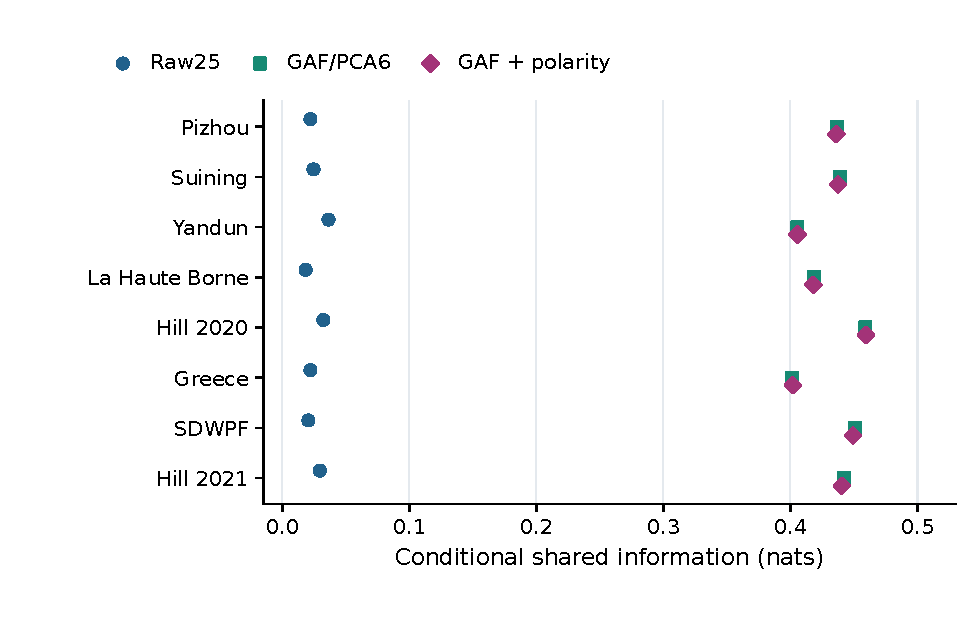
\includegraphics[width=\linewidth]{fig06_conditional.pdf}
\caption{Shared geometry after conditioning on protocol pair, direction, amplitude, duration and pre-window power. Values subtract the mean within-stratum permutation reference. The near-overlap of the angular variants shows similar geometry under these controls. Protected polarity targets directional information, tested with independent wind measurements in the following figures; it is not selected to maximize this conditioned score.}
\label{fig:main6}
\end{figure}

\subsection{Protected polarity preserves a physically meaningful distinction}\label{protected-polarity-preserves-a-physically-meaningful-distinction}

For the signed-domain Gramian angular summation field (GAF) used here, a path and its sign reversal produce the same image. Fig.~\ref{fig:main7} shows the paired paths and Fig.~\ref{fig:main8} shows their identical angular field. This identity gives a precise intervention: one sign bit at a nonzero reference coordinate resolves the ambiguity of the full field. For a compact representation, we retain five coordinates from principal component analysis (PCA) and reserve a sixth coordinate for polarity. This protects the directional distinction through compression; exact recovery of the entire path is a property of the full field plus sign, whereas the compressed representation is evaluated empirically. The next experiment tests the physical value of retaining that distinction.

\begin{figure}[H]
\centering
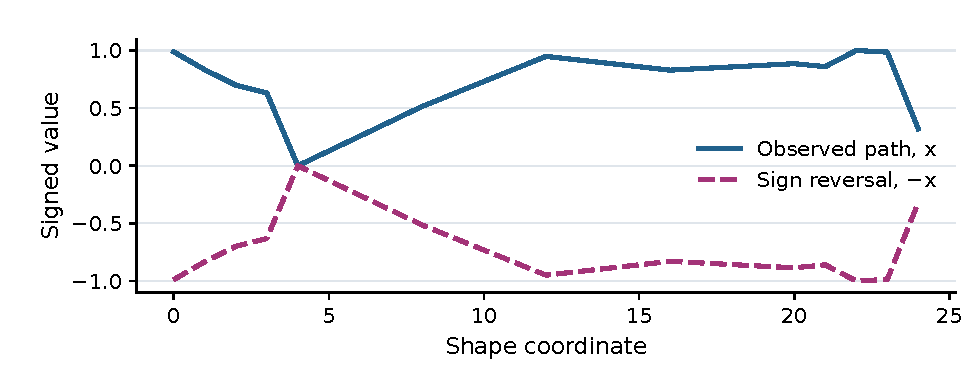
\includegraphics[width=\linewidth]{fig07_polarity_paths.pdf}
\caption{An observed 25-coordinate path and its controlled global sign reversal. These two paths have opposite polarity and the same signed-domain Gramian angular summation field.}
\label{fig:main7}
\end{figure}

The empirical comparison separates preserving a coordinate from appending an input channel. Appending signed coordinates before PCA exposes them to the same compression as the image. Reserving a polarity coordinate after PCA keeps the chosen distinction explicit. Both representations remain compact, but they encode different guarantees about directional information.

\begin{figure}[H]
\centering
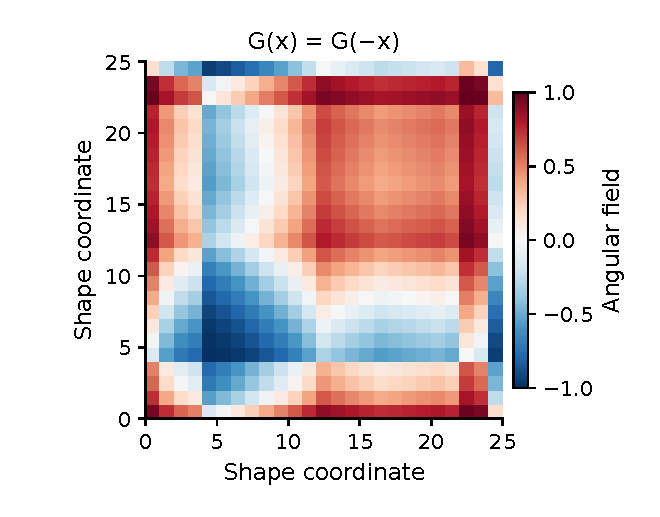
\includegraphics[width=.66\linewidth]{fig08_shared_gasf.pdf}
\caption{The common Gramian angular summation field for the two paths in Fig.~\ref{fig:main7}. The identity G(x)=G(−x) motivates retaining a sign coordinate alongside the compressed angular representation.}
\label{fig:main8}
\end{figure}

In the primary fit, the protected polarity coordinate has a variance share bounded above by approximately 0.225\% in the six-dimensional encoding. Its small geometric weight explains the similar cluster partitions; its scientific role is to retain a direction that can be read by a supervised physical head.

The compact comparison contains six-dimensional ordinary GAF/PCA, signed-channel GAF/PCA, protected-polarity GAF/PCA and raw/PCA. Raw25 and the nine-statistic representation provide explicit higher-dimensional references. All variants use the same training events and weather targets, with shared downstream model-selection budgets. This comparison tests whether an explicit polarity coordinate supplies useful directional information at a fixed six-dimensional representation budget.

Five regional-weather evaluations relate these event representations to signed 100-m wind-speed change. At Hill of Towie, the protected-polarity representation reduces held-out signed log loss from 0.379 to 0.345, a 9.03\% reduction, with a seven-day block interval of 6.35--10.96\%. Decomposing the same probability score into occurrence and direction components explains the gain. Conditional wind-tendency AUROC rises from 0.538 to 0.932, while the occurrence component changes little. The intervention principally restores the distinction that its mathematical construction was designed to preserve.

The five evaluations are Pizhou, Suining, Yandun, La Haute Borne and Hill of Towie. At Hill, the occurrence component is 0.307 for GAF/PCA and 0.311 for protected polarity, whereas the direction component falls from 0.073 to 0.034. The gain is therefore directional information rather than a change in event frequency.

Continuous shape and scalar metadata provide a second route to process information. Adding raw25 to direction, amplitude, duration, initial power and pre-window power reduces signed regional-weather log loss pointwise at all five sites. The complete block intervals and the corresponding hard-cluster-label probes are reported together in the Supplementary Information. This comparison separates the information in a trajectory from the coarser information carried by a four-class label.

Prototype geometry provides a compact bridge between these descriptions. Adding distances to the four frozen raw25 prototypes improves signed-weather log loss pointwise at all five sites. At Yandun, the four-distance input reduces log loss by 0.0152 nats beyond the scalar controls. Retaining graded location within the learned structure therefore supports a physical-probability interface while preserving a compact four-coordinate description.

\subsection{Independent LiDAR validates directional information recovery}\label{independent-lidar-validates-directional-information-recovery}

To test the external validity of protected polarity, we use independent 2026 LiDAR measurements. Fig.~\ref{fig:main9} places the two instruments on one ROC canvas. A ground-based instrument near T11 measures horizontal wind near hub height, and a nacelle instrument on T07 measures upstream flow at a 208-m range. Applying the frozen Hill-2020 physical probes gives 5,106 and 2,627 matched events with complete wind support at the primary clock alignment. Protected polarity reduces signed log loss relative to angular PCA by 7.21\% at T11 and 9.20\% at T07. The respective seven-day block intervals are 5.37--8.85\% and 7.42--10.72\%; both gains also retain their direction under the predeclared ±10-min clock checks.

A separate chronological field-calibration experiment translates the source scores into local probabilities. Calibration training ends before 14 March, validation ends before 7 April, and testing uses later events with their full contexts contained in the test period. The three-class test contains 1,064 T11 and 444 T07 events. Directional AUROC uses the 705 and 285 events with measured wind increase or decrease, respectively, occupying four seven-day blocks at each instrument. Protected polarity attains AUROC 0.890 (95\% block interval 0.822--0.974) and 0.905 (0.808--0.947), compared with 0.494 (0.468--0.544) and 0.477 (0.321--0.599) for angular PCA. Three-class signed log loss decreases by 16.42\% and 16.11\%, respectively. The independent measured outcome thus identifies a useful physical distinction in the event representation. ARI and AUROC answer different questions: ARI measures agreement between partitions of matched events; AUROC measures discrimination of independently measured wind tendencies.

\begin{figure}[H]
\centering
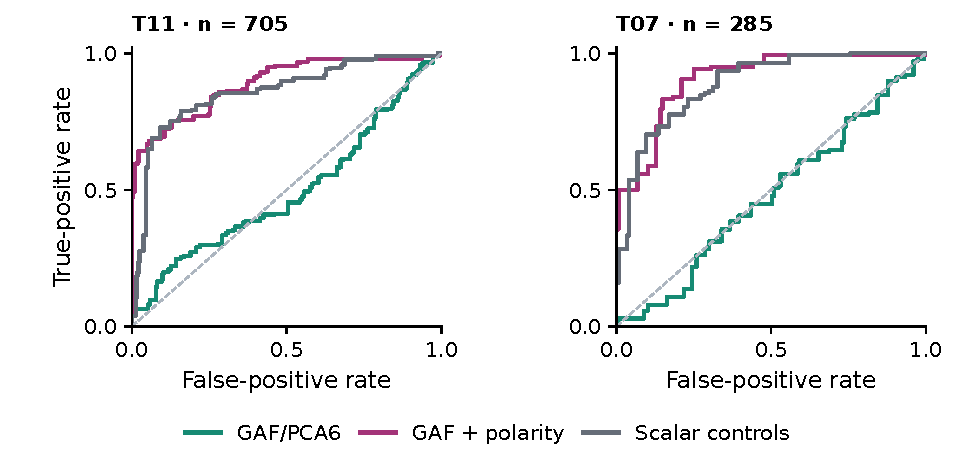
\includegraphics[width=\linewidth]{fig09_lidar_roc.pdf}
\caption{Independent LiDAR direction discrimination after chronological calibration. T11 and T07 occupy the left and right panels, with 705 and 285 measured increase/decrease events. Small-net-change observations are retained in the separate three-class score. Both instruments use the same representation colors and axes.}
\label{fig:main9}
\end{figure}

This experiment answers the reverse-identification question directly: an observed power-event description can support a probability for an externally measured wind-speed tendency. The temporal ordering in this task is retrospective process identification. Its forecasting counterpart uses information available at issue time to predict future event probabilities, as tested in the next section.

\subsection{A second instrumented field archive preserves the event interface}\label{a-second-instrumented-field-archive-preserves-the-event-interface}

SMARTEOLE supplies a second public instrumented wind farm: seven Senvion MM82 turbines, 1-min supervisory control and data acquisition (SCADA), a ground WindCube profiler and a yaw-control log. Fig.~\ref{fig:main10} combines its physical transfer with the resampled LiDAR distributions. Applying the frozen Pizhou K-means (k=4, seed 41) transformations after complete 30-min aggregation produces 77 supported turbine-by-configuration-pair rows, containing 8,985 matched primitive-event pairs per representation summary. Raw25 reaches median ARI 1.000 on this high-support subset; 45 of the 77 rows have ARI=1.000, while the pair-weighted ARI is 0.964 and the all-row pair-weighted ARI is 0.887 across 852 rows. GAF/PCA and protected polarity reach 0.605 and 0.597 on the same supported-row summary. Here agreement refers to the retained partition on matched events. Reporting the support rule and weighted diagnostics makes the transfer result transparent: the high-support raw25 median is a concentrated structural-transfer signal, not an identity claim for every detector pair. The structural result establishes a working transfer of the event ledger and one-to-one correspondence interface to a different field archive.

The same frozen Pizhou physical heads use WindCube 80-m endpoint wind-speed changes as an independent outcome. Across the seven turbines, models combining scalar event descriptors with raw25 attain direction AUROC from 0.902 to 0.926. Corresponding angular and protected-polarity models retain the same scalar inputs, including direction, to evaluate shape information under a common control set. The SMARTEOLE provider removes rows with at least one stopped turbine, so this experiment identifies structure and wind-process information during the supplied operating population.

\begin{figure}[H]
\centering
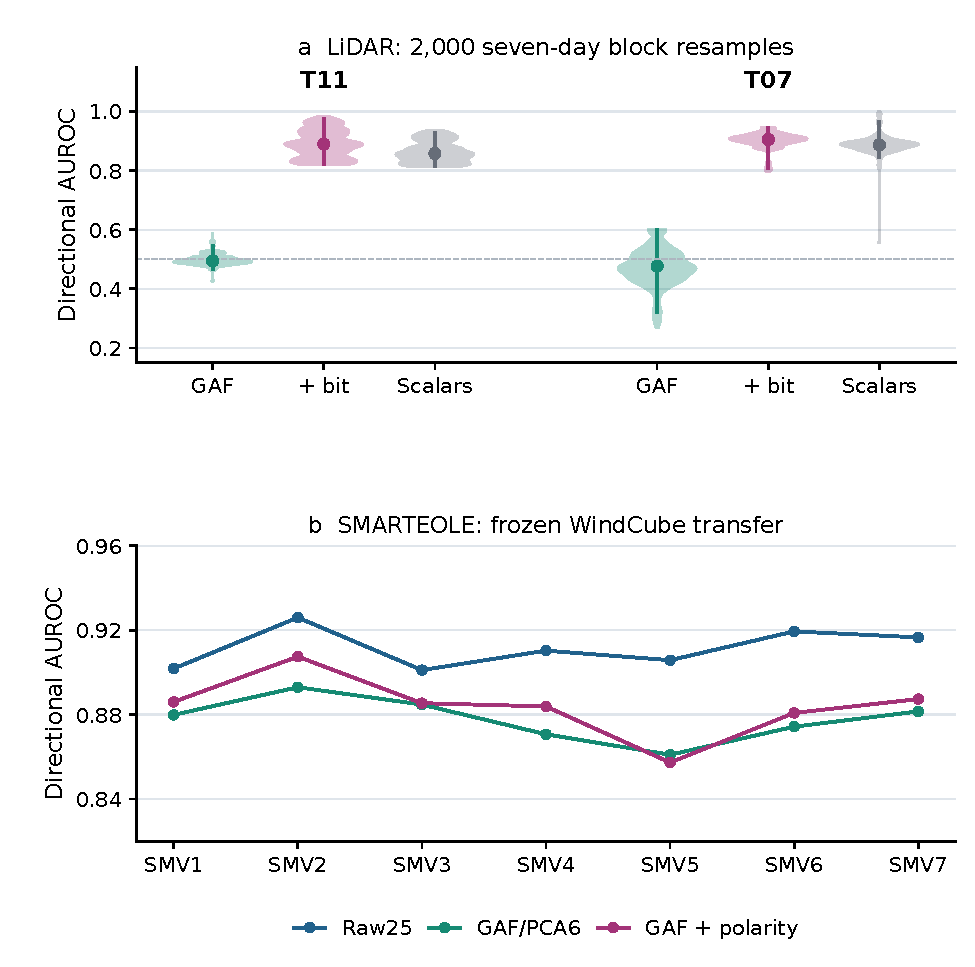
\includegraphics[width=\linewidth]{fig10_external_validation.pdf}
\caption{External physical validation across two instrumented fields. Top: empirical directional-AUROC distributions from 2,000 resamples of four occupied seven-day blocks per Hill instrument; bars show percentile intervals and dots medians. Bottom: seven turbine responses paired with the same SMARTEOLE WindCube reference, with scalar controls shared across representations. SMARTEOLE structural agreement has a raw25 median of 1.000 across 77 high-support rows, of which 45 equal 1.000; pair-weighted ARI is 0.964 and all-row pair-weighted ARI is 0.887. Structural row distributions are supplied separately.}
\label{fig:main10}
\end{figure}

\subsection{Human reference and controlled localization connect structure to detection}\label{human-reference-and-controlled-localization-connect-structure-to-detection}

The human reference adds three independent assessments of 320 windows from eight archives, with 40 windows per archive. Review targets were the central two hours of a four-hour display. Nominal Krippendorff's alpha is 0.528 for event presence (95\% seven-day block interval 0.455--0.599) and 0.476 for dominant morphology (0.426--0.523). With the seventeen detector configurations fixed before receipt of these labels, the 120-min threshold detector attains F1 values of 0.822, 0.808 and 0.838 against the three observers. The three independent readings provide a human reference for recognizable production changes while preserving observer-level variation rather than imposing a consensus label.

The detector contrasts describe operating choices across the three references. The 60-min threshold has higher precision and lower recall, whereas the 240-min threshold has higher recall and lower precision. The 0.10 endpoint corridor produces F1 values of 0.833, 0.860 and 0.787, making the precision--recall trade-off explicit. The three-way alpha is lower than the earlier two-observer estimate because the third observer uses a different mixture of V, inverted-V and oscillatory labels; the observer identifiers remain anonymous, so the difference is interpreted as reference variability rather than an observer-specific mechanism. Presence-level F1 supplies the primary detection reference, while morphology agreement supports auxiliary shape interpretation. All seventeen configurations and observer-level results are retained in the Supplementary Information.

Structural survival and physical tracking answer different questions from event localization. We therefore retain the earlier controlled episode benchmark as a task-level validation. Synthetic 96-point trajectories contain known event support, direction, amplitude and shape. TimesNet, KAN-AD (Kolmogorov--Arnold network anomaly detection), a temporal convolutional network (TCN) autoencoder and a positional Transformer autoencoder receive the same training sequences and score-to-interval budget. Threshold calibration and event grouping are evaluated as separate output steps.

At fixed model scores, calibration followed by grouping increases F1 from 0.263 to 0.609 for TimesNet and from 0.306 to 0.642 for KAN-AD. A validation-selected KAN-AD configuration reaches mean F1 0.795 across three seeds on the existing test population. On fresh post-selection sequences, KAN-AD reaches F1 0.793 versus 0.732 for the fixed mean-change rule; in a higher-noise condition it reaches 0.646 versus 0.367. This experiment demonstrates why a dynamic-event benchmark evaluates both the score model and the rule that turns scores into intervals. It also supplies event-level precision, recall and F1 alongside matched-structure agreement. These synthetic localization comparisons evaluate how a score becomes an event interval (Fig.~\ref{fig:main11}).

\begin{figure}[H]
\centering
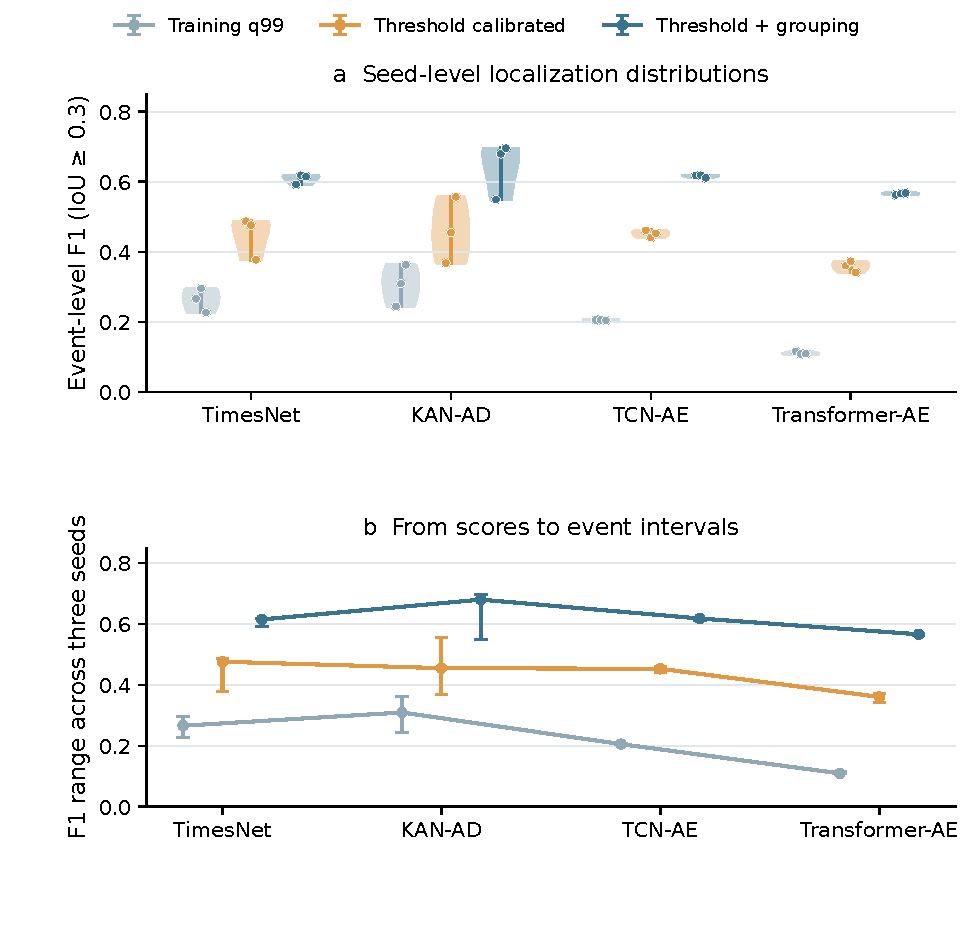
\includegraphics[width=\linewidth]{fig11_localization.pdf}
\caption{Event-level localization after score calibration and interval grouping. The upper panel shows the three archived seed values as a compact violin and point distribution; the lower panel compares the corresponding median and min--max range across seeds. The grouping rule is evaluated at a fixed IoU threshold, so it measures the complete score-to-interval interface rather than the anomaly score alone.}
\label{fig:main11}
\end{figure}

\subsection{High-ramp periods concentrate settlement exposure}\label{high-ramp-periods-concentrate-settlement-exposure}

The decision experiment evaluates six forecasting variants for 1-, 2- and 4-h horizons on Hill of Towie aggregate power. The information sets add observed wind, available historical events, and predicted future-ramp probabilities. The latter probabilities gate three regression experts. Historical-event inputs are counts and proportions of the four frozen raw25 clusters over the preceding four hours. This economic track therefore tests raw25-based event information; the angular and protected-polarity comparisons belong to the physical-information track. Models use completed observations at issue time, and archived Elexon half-hour prices---the UK Balancing and Settlement Code (BSC) system prices---score the resulting energy deviations.

{\def\LTcaptype{none} % do not increment counter
\begin{longtable}[]{@{}
  >{\raggedright\arraybackslash}p{(\linewidth - 2\tabcolsep) * \real{0.5000}}
  >{\raggedright\arraybackslash}p{(\linewidth - 2\tabcolsep) * \real{0.5000}}@{}}
\toprule\noalign{}
\begin{minipage}[b]{\linewidth}\raggedright
Forecast variant
\end{minipage} & \begin{minipage}[b]{\linewidth}\raggedright
Information added to power history and calendar
\end{minipage} \\
\midrule\noalign{}
\endhead
\bottomrule\noalign{}
\endlastfoot
Persistence & Latest completed aggregate power, used directly \\
Power + calendar & Learned mapping from completed power history and calendar \\
Observed weather & Completed turbine-wind history \\
Historical events & Available raw25-cluster counts and proportions \\
Ramp mixture + observed weather & Predicted ramp probabilities from observed weather gate three experts \\
Ramp mixture + historical events & Historical-event inputs augment the weather-based ramp mixture \\
\end{longtable}
}

Large changes concentrate exposure. Fig.~\ref{fig:main12} shows that periods with a power change of at least 20\% of the 48.3-MW fleet capacity occupy 17.8\%, 24.8\% and 34.0\% of evaluated targets at the three horizons, yet account for 53.7\%, 63.8\% and 70.5\% of gross imbalance debits. The associated ramp-subset normalized mean absolute errors (nMAEs) are 32.4\%, 34.7\% and 37.5\%, compared with whole-period values of 11.0\%, 13.7\% and 17.5\%. The exposure concentration identifies the periods in which event-aware information can carry the greatest operational relevance.

\begin{figure}[H]
\centering
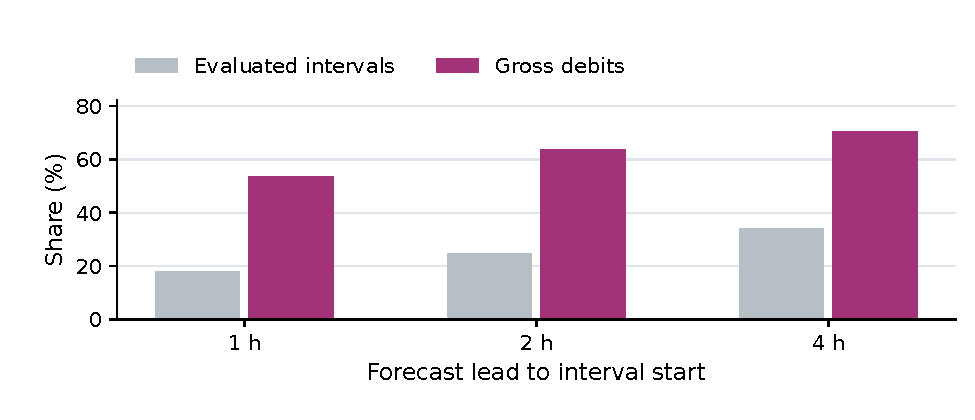
\includegraphics[width=\linewidth]{fig12_ramp_exposure.pdf}
\caption{Large-ramp periods concentrate settlement debit exposure. Grey bars show the eligible interval share with at least 20\% fleet-capacity change; magenta bars show their share of persistence gross debits on the same targets and observed prices.}
\label{fig:main12}
\end{figure}

The predicted-ramp experiment provides a concrete information pathway. Fig.~\ref{fig:main13} places forecast error and observed-price exposure in aligned panels. At 2 h, adding available historical-event information to the otherwise matched ramp-mixture model changes nMAE from 14.69\% to 14.47\% and gross imbalance debits from £292,263 to £279,178. A fixed-budget residual-forecast matrix then fits 48 validation-defined candidates, including absolute- and squared-error objectives, ramp weights and persistence blends. The selected weather-plus-event model reduces nMAE from 14.47\% to 13.69\% and gross debits from £279,178 to £233,084 in the reused 2-h test calendar. Relative to the legacy ramp model, the gross-debit reduction is 16.51\% (7-day block interval 11.39--22.31\%) and the nMAE reduction is 0.79 percentage points (0.40--1.22). This is an exploratory fixed-matrix extension on the existing test period; its value is to show how protocol-preserved event information can be combined with a decision-aligned forecast objective. Forecast accuracy, gross debits and net settlement cashflow remain separate evaluation quantities because positive and negative deviations are priced and settled differently.

\begin{figure}[H]
\centering
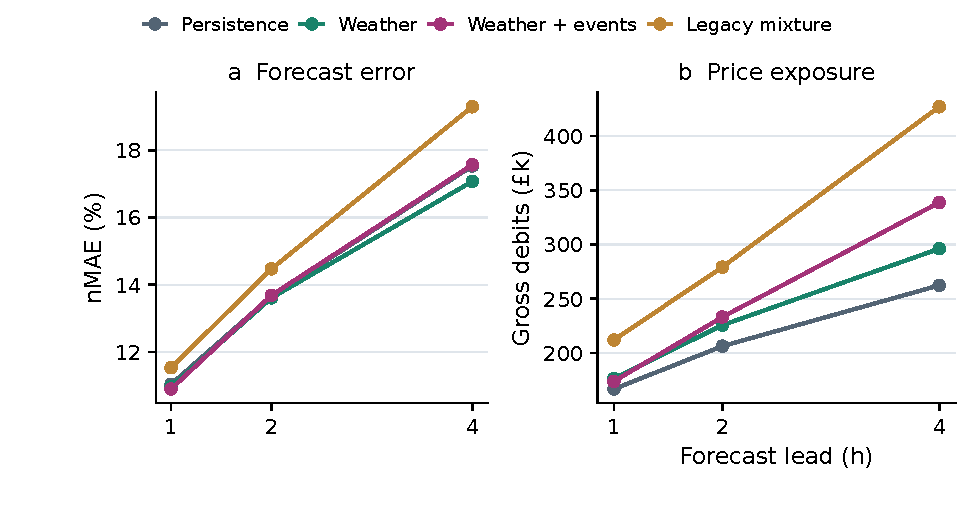
\includegraphics[width=\linewidth]{fig13_forecast_cost.pdf}
\caption{Forecast error and gross imbalance debits at 1-, 2- and 4-hour leads. Left and right panels use the same model colors and common eligible test targets within each horizon. Forecast candidates were selected on validation nMAE; the reused test calendar is exploratory. Both weather-only and persistence baselines accompany the event-aware forecast.}
\label{fig:main13}
\end{figure}

The earlier Pizhou/Yandun fleet benchmark supplies a second task-level check. Increasing the ramp weight from 0 to 4 reduces TCN ramp-subset nMAE from 35.45\% to 32.57\% in Pizhou and from 36.52\% to 33.21\% in Yandun, while whole-period nMAE rises from 7.74\% to 8.63\% and from 8.36\% to 10.08\%, respectively. The result makes the decision trade-off explicit: an objective can target the rare, expensive ramp population while moving the aggregate score in the opposite direction.

The mathematical relationship explains why this separation is necessary. Two forecasts can have identical nMAE and different threshold-exceeding errors; identical errors can also incur different costs at different prices. For an illustrative scale in British pounds (GBP), a 30-MW shortfall sustained for 1 h corresponds to 30 MWh, or GBP 15,000 at GBP 500 per MWh. This example uses GBP throughout and involves no currency conversion. Actual cost depends on the time-resolved errors and the applicable settlement or assessment formula. Gross debits measure expenditure exposure; signed settlement cashflow includes both debits and credits. Profitability additionally requires contractual revenue and asset costs.

Storage is evaluated through a common-commitment experiment: every information arm receives the same persistence commitment when an issued forecast is available, with a zero-correction fallback when it is unavailable, uses the same inventory controller and returns to the same daily terminal state of charge. Observed prices score all 3,504 test half-hours; issued forecast availability is recorded for 2,794 of them using issue-time feature readiness. This construction isolates the operating cashflow attributable to the controller's information while holding contractual revenue fixed. The full capacity frontier and validation-selected choices appear in the Supplementary Information.

The metered-correction capability replay adds a physically feasible ex-post storage capability result. Fig.~\ref{fig:main14} reports the settlement debit and signed-cost response side by side. At the two-hour horizon on 58 complete test days, an event-aware schedule paired with a battery rated at 20\% of farm capacity reduces gross debit from £223,345 to £162,784 (27.1\%; seven-day block interval 23.95--30.73\%) and reduces settlement credits from £166,150 to £91,709. The replay uses the observed Elexon single-price calendar, with its buy-side and sell-side columns checked to be identical; signed settlement cost changes from £57,195 to £71,075 because the correction changes purchase and sale volumes and settlement includes the restoration actions required to return terminal inventory. In the 2,784 test intervals, 2,582 have an issued event-aware forecast and the remainder use the persistence fallback. This separates a large reduction in high-ramp exposure from the contract-dependent question of net profitability. The benchmark uses the realised current half-hour power measurement and therefore quantifies correction capability rather than issue-time forecast gains; future power and future prices remain unavailable.

\begin{figure}[H]
\centering
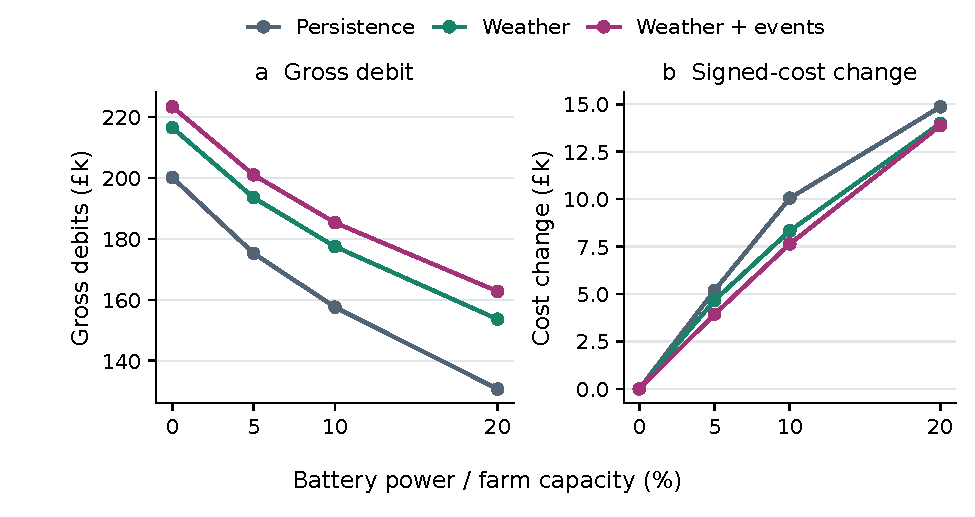
\includegraphics[width=\linewidth]{fig14_storage.pdf}
\caption{Physically feasible ex-post correction capability under observed single-price settlement over 58 complete test days. The benchmark observes the realised half-hour mean and applies a power- and SOC-constrained correction, including settlement of the actions required to restore daily terminal inventory; it is not an issue-time forecast gain. Left: gross debits after correction, with a separate baseline for each model schedule. Right: signed settlement cost change for each model-specific schedule; positive values indicate higher signed cost. The 20\%-power event-aware case reduces gross debit by 27.1\% while its signed cost increases, because settlement credits fall by more than debits.}
\label{fig:main14}
\end{figure}

The decision surface separates forecast-information value from asset-investment value. Historical event information improves two-hour error and gross-debit exposure in the matched ramp-mixture comparison. A profitable storage investment additionally depends on contractual revenue, capital and cycling costs, permitted services and the local price mechanism. The common-commitment forecast-only controller and the metered-correction frontier answer different operational questions: the first tests issued information, while the second quantifies how an installed battery can convert current metering into lower settlement exposure. The policy bridge is explicit rather than cosmetic: Jiangsu rules require 15-min submitted curves, EMS assessment and monthly treatment of unqualified points, while the RTE framework assigns half-hourly imbalance settlement through the responsible party's sign, system trend, VWAP and coefficient k \citep{rtesettlement}. Supplementary Table S55 records these requirements and the missing station-level inputs needed for a faithful jurisdictional replay.

\FloatBarrier
\section{Discussion}\label{discussion}

This study establishes event measurement as a link between power trajectories, physical-process information and operational evaluation. Its central result is constructive: event descriptions can be designed to preserve the distinctions needed for a task, and those distinctions can be tested against independent observations. The four-layer framework supplies the comparison interface; the polarity intervention supplies an explicit information-preserving mechanism; the LiDAR experiment demonstrates a corresponding physical discrimination gain.

The ordered and angular representations reveal why a single clustering score is an incomplete design objective. Ordered partitions retain polarity strongly. Angular partitions retain substantial conditioned geometry. A protected polarity coordinate combines a useful invariance with an explicitly retained physical distinction. This principle extends beyond the particular encoder: identify a task-relevant equivalence introduced by a representation, preserve the necessary distinguishing information, and evaluate the resulting description on an external outcome. The nearest-prototype margin provides a complementary local criterion for assignment stability.

Coarse classes and calibrated probabilities serve different roles. A cluster label is a useful summary of a recurring trajectory, while a physical-process probability quantifies what that trajectory suggests about an external measurement. In the five-site tests, adding a hard four-class label to scalar metadata gives small, heterogeneous incremental gains. Continuous event information is richer. The source probabilities also require field calibration when transferring from regional reanalysis to local LiDAR. Together these observations motivate an event interface containing shape, metadata, prototype membership and calibrated task probabilities, with each component evaluated for its intended use.

The economic results provide an operational interpretation of event information: large changes concentrate settlement exposure, and available historical structure can improve a ramp-conditioned forecast. Capacity selection answers a further question. In the tested single-price common-commitment case, validation selects zero incremental storage for every information arm. This result describes the marginal value of adding a battery to the tested controller and commitment; it does not describe whether an operating wind farm owns storage or whether storage is useful for other services. The capacity frontier shows the operating-cost change for 5--20\% power fractions, allowing existing assets to be evaluated under their own capital, contract and reserve conditions. Event information improves exposure and error descriptions, whereas profitability also requires capital costs, contractual positions, grid permissions and the applicable local price mechanism.

\subsection{Limitations and scope conditions}\label{limitations-and-scope-conditions}

Structural conclusions refer to matched, encodable events, with their coverage and support reported. Regional-weather and LiDAR relationships establish external association and probabilistic discrimination; causal effects of weather or operation require a supported intervention design. Hill control records and SCADA-based yaw indicators offer routes to mechanism analysis, with control execution, transition periods and wake interference requiring separate checks. Greece and SDWPF contribute structural tests; independent weather matching awaits verified absolute clock and location information.

The 320-window reference contains three independent observers' assessments of central-region presence and dominant morphology. Region-level agreement is quantified before any adjudication; event-boundary errors and onset delay require corresponding reference labels. The earlier 120-region review remains a separate cohort. The 2026 LiDAR calibration was developed after the frozen transfer analysis and is an exploratory chronological test with four seven-day blocks per instrument in its final period. SMARTEOLE extends the field setting, while its provider's operating-period filter defines the available population. Additional calibration periods and instrumented sites will test the persistence of these relationships.

The completed observed-price evaluation concerns Great Britain. Formal Chinese documents define 15-min submitted forecasts, EMS-based assessment, monthly unqualified-point treatment and exemption records; the required station-level inputs are not available for a faithful fee replay. RTE defines settlement by the sign of the balance-responsible-party imbalance and an interval-specific positive or negative imbalance price \citep{rtesettlement}, but the historical French price series and perimeter are not aligned with La Haute Borne. The present monetary results therefore use the acquired Elexon series. Chinese and French policy sources specify reproducible transfer simulations rather than realized invoices. Public release of the current event package also remains subject to source-specific permissions and attribution.

The framework gives the community a concrete reporting and benchmark target. An event result should carry its physical-time protocol, matched population, task-relevant information and decision horizon. Benchmark tracks should separately score structural survival, event localization, independent-process tracking and forecast-to-cost performance. This separation rewards measurements that are useful for a stated scientific or operational purpose, and provides a reusable route from event discovery to physical interpretation and dispatch research.

\FloatBarrier
\section{Methods}\label{methods}

\subsection{Data and common observation conditions}\label{data-and-common-observation-conditions}

The study includes Pizhou (33 turbines), Suining (14), Yandun (117), La Haute Borne (4), Hill of Towie (21), Greece (10) and SDWPF (134). Chinese archives contribute 298 turbines and European archives 35. La Haute Borne is associated with the OpenOA data ecosystem \citep{perr-sauer2021openoa}; the Greek and SDWPF archives supply independent public monitoring resources \citep{greece2024, sdwpfdata}. The main source periods are September 2023--February 2025 for Pizhou, September 2023--August 2024 for Suining, February--August 2024 for Yandun, 2014--2015 for La Haute Borne, 2020 for Hill of Towie, January--June 2020 for Greece and 2020--2021 for SDWPF. Hill of Towie 2021 January--June supplies the frozen temporal evaluation, and its 2026 measurements supply the instrumented physical test \citep{hill2026data}. ERA5 denotes the European Centre for Medium-Range Weather Forecasts fifth-generation reanalysis.

Complete native observations form each half-hour average. Explicit missing bins separate valid runs. SCADA interval-end timestamps at Hill of Towie are shifted to interval starts. A chronological 60/20/20 split defines fitting, validation and test periods. Main detector normalization uses each turbine's training-period q99.5 power, expressed as a production scale. The same empirical method is used for Pizhou and Greece; fitted transformations remain separate from evaluated data \citep{leakage2023}. Nameplate capacity supplies physical MW units where verified, including the 21 × 2.3-MW Hill fleet. Event contexts remain within one split and valid run.

\subsection{Protocol space and event hierarchy}\label{protocol-space-and-event-hierarchy}

Let a protocol be \(\pi=(Q,D,M,F,C)\), where \(Q\) specifies clock, sampling, quality and amplitude calibration; \(D\) constructs intervals; \(M\) establishes correspondence; \(F\) encodes trajectories; and \(C\) assigns structure. A controlled comparison changes an identified component while retaining the remaining conditions. Structural agreement is estimated on the matched, encodable population. Weather-risk and economic estimands use their eligible calendar populations.

The complete experiment map is provided in Supplementary Table S0. It records the data period, analysis unit, purpose and status of each catalogue, transfer, physical-process, forecast and cost experiment, so that the structural, physical and decision estimands remain distinct.

The seventeen detector configurations include fixed-amplitude changes, historical financial tails, adjacent-mean changes, fixed and adaptive corridors, the Swinging Door Algorithm (SDA) and the 2015 conference Optimized Swinging Door Algorithm (OpSDA) formulation \citep{florita2013, cui2015}. Nominal lags are 60, 120 and 240 min. Historical tails use a 24-h preceding window with a 0.10 minimum amplitude and 0.05/0.95 quantiles. Threshold and mean-shift configurations use 0.20 relative power in the main analysis. The adaptive corridor sets and freezes its width at each segment start from available past differences. Composite intervals join adjacent opposite legs, retain child identifiers and record a measured internal turning point, with a four-hour primary extent.

\subsection{Correspondence and structure scores}\label{correspondence-and-structure-scores}

For positive-duration intervals \(I_a=[s_a,e_a)\) and \(I_b=[s_b,e_b)\), let \(J=\max(0,\min(e_a,e_b)-\max(s_a,s_b))\) and \(U=(e_a-s_a)+(e_b-s_b)-J\). The intersection over union (IoU) is

\[
\operatorname{IoU}(I_a,I_b)=J/U,\qquad U>0.
\]

The implementation rejects zero-duration and reversed intervals (e≤s) before overlap calculation. A zero union is an invalid comparison and receives no score or edge. Empty catalogues contain no matches and their coverage is undefined; intervals touching only at an endpoint have IoU=0. For overlapping valid intervals, U equals the enclosing duration used by the implemented candidate-edge calculation. Matches share site, turbine, split and hierarchy. Greedy assignment sorts feasible edges by descending IoU with deterministic tie rules, using IoU ≥ 0.5. If N\_a and N\_b are the eligible event counts and M is the number of one-to-one matches, left and right coverage are M/N\_a and M/N\_b. Primary summaries use supported, informative configuration pairs common to all six representations and three seeds, first taking the median across seeds within each pair and then across pairs. ARI \citep{hubert1985} and normalized mutual information (NMI) quantify partition agreement. Constant partitions and pairs with fewer than 100 matches remain in separate support tables.

The many-to-many extension builds a bipartite graph for each site, turbine, test split and configuration pair. All edges satisfying IoU ≥ 0.5 are retained, with 0.3/0.7 sensitivities. Connected components classify one-to-one, one-to-many, many-to-one and many-to-many correspondence. A primitive-only arm keeps the original event population; a hierarchy-inclusive arm allows primitive intervals to correspond to composite V/inverted-V episodes. Coverage counts unique connected nodes on each side, never edge multiplicity. Each component receives one vote when comparing label composition: if p\_a and p\_b are its four-class frequency vectors, composition overlap is sum\_j min(p\_aj,p\_bj). This descriptive score preserves mixture proportions, while within-component temporal order is represented by the stored intervals and turning points. It is distinct from ARI. A separate containment sensitivity uses intersection/minimum duration ≥ 0.5, allowing a short leg to belong to a longer episode. Components longer than four hours remain explicitly counted as linked measurement supports. Shared seven-day calendar blocks anchor each component at its earliest start; 2,000 draws quantify conditional temporal variation. Per-event predictions use the frozen Pizhou raw25 k=4 seed-41 model.

Configuration names fix the left/right order lexicographically. A supported component pair contains at least 100 connected components; this count is descriptive and does not filter the all-configuration site summary. Site composition scores and topology proportions weight components equally across all 136 configuration pairs. Pooled coverage divides total unique connected nodes by total eligible nodes across those comparisons; an event can contribute once within each comparison. The main one-to-one coverage table instead averages the 136 configuration-specific fractions equally. An exact count reconciliation confirms identical primitive populations and one-to-one matches under both summaries (coverage\_aggregation\_reconciliation.csv).

\subsection{Representations, clustering and information preservation}\label{representations-clustering-and-information-preservation}

A shape has four pre-event coordinates, seventeen interpolated internal coordinates and four post-event coordinates. Let p\_j denote these sampled power values and p\_s the event-start power. We formed x\_j=(p\_j−p\_s)/a with a=max\_j\textbar p\_j−p\_s\textbar{} over all 25 coordinates, requiring a\textgreater0 and finite values. Hence x belongs to {[}−1,1{]}\^{}25; zero-variation supports were ineligible for shape analysis. This per-event normalization retains sign and temporal geometry, while amplitude, duration and initial power remain explicit metadata. Context locations preserve physical time across sampling grids. The six representations are raw25, statistics9, raw/PCA6, GAF/PCA6, signed-channel GAF/PCA6 and GAF/PCA5 plus polarity. K-means at k=4 is the primary analysis; k=2/6 and Gaussian-mixture/medoid comparisons use the same training budget and frozen test events.

For the finite signed unit-domain vector x, set \(c_i=\sqrt{1-x_i^2}\ge0\). The Gramian angular summation field (GASF), the GAF variant used here, is \(G=xx^T-cc^T\) \citep{wang2015gaf}, equivalent to \(G_{ij}=\cos(\arccos x_i+\arccos x_j)\). For an exact, uncompressed full field, its diagonal yields \(|x_i|=\sqrt{(G_{ii}+1)/2}\), and \(G+cc^T=xx^T\). Choose an anchor r with \(|x_r|>0\); the sign bit \(b=\operatorname{sgn}(x_r)\) gives \(x_r=b\sqrt{(G_{rr}+1)/2}\) and \(x_i=(G+cc^T)_{ir}/x_r\). The deterministic largest-magnitude anchor, with the first index breaking ties, is recoverable from the diagonal. The all-zero path is already determined, although constant supports are excluded by preprocessing. This recovers the normalized trajectory; restoring absolute power also requires its offset and scale. PCA retains only part of the field, so GAF/PCA5 plus polarity is an empirical six-dimensional representation, not an exact-inversion guarantee. It preserves the anchor sign explicitly and is evaluated on held-out clustering and physical targets.

For fixed Euclidean prototypes, let \(m\) be the distance to the second closest prototype minus the distance to the closest. A representation perturbation of norm less than \(m/2\) preserves the closest assignment by the triangle inequality. This supplies a local stability condition within a shared representation space.

Conditional information analysis stratifies configuration pair and training-defined physical descriptors. Individual analyses condition on direction, amplitude, duration or pre-window power; the joint analysis combines coarse scale strata and both event directions. Strata require at least thirty pairs. One hundred within-stratum, within-turbine permutations quantify the chance contribution under the preserved controls. Conditional mutual information, remaining label entropy and retained support are reported together.

For matched-event partition labels \(L_a,L_b\) and conditioning stratum \(W\), we calculated

\[
I(L_a;L_b\mid W)=\sum_w p(w)\sum_{a,b}p(a,b\mid w)
\ln\frac{p(a,b\mid w)}{p(a\mid w)p(b\mid w)}.
\]

The reported excess is the observed value minus the mean within-stratum permutation value. Descriptor cut points were fitted on Pizhou training events: individual analyses used terciles, and the joint analysis used median splits for amplitude, duration and starting power together with both event directions. All information and permutation calculations used retained matched pairs.

\subsection{Physical reference and probability experiments}\label{physical-reference-and-probability-experiments}

Hourly ERA5 wind, temperature, pressure and related surface fields provide regional context for five geographically aligned archives \citep{hersbach2020, era5docs}. The event-level physical target is \(\Delta u=u_{100}(e)-u_{100}(s)\), classified as decrease for \(\Delta u\le-1.5\) m s−1, increase for \(\Delta u\ge1.5\) m s−1, and small net change otherwise; event duration satisfies \(0<e-s\le4\) h. The ±1.5 m s−1 cutoffs are study-defined symmetric contrast levels, fixed for the regional probe before the later LiDAR transfer. They provide a common operational definition of a substantial endpoint wind-speed tendency, rather than a turbine cut-in/cut-out boundary or a universal meteorological ramp threshold. The four-hour limit matches the longest principal detector horizon and the composite-event window used in this study, focusing the probe on intraday dynamics. It does not require every wind change to span four hours: the same endpoint contrast may occur over a shorter event. A V-shaped excursion may return to small net change while retaining substantial internal variation, which is evaluated through event morphology and the overlap analysis. NOAA Integrated Surface Database (ISD) observations are archived with variable-level quality codes and precipitation accumulation duration \citep{noaaisd}; independent LiDAR supplies the local-wind test.

Physical probes share training-event identifiers and two gradient-boosted-tree leaf budgets. Training fits the model; validation selects leaf budget and probability temperature. Scalar controls are direction, amplitude, duration, starting power and pre-window mean. Standalone representations, scalar-plus-representation inputs and scalar-plus-hard-cluster inputs form distinct comparisons. Proper log and Brier scores evaluate probabilities \citep{gneiting2007}. Log-score differences estimate model-usable predictive information.

The 2026 instrument test uses 58-m horizontal wind from ZX300 unit 2428 near T11 and 208-m fit-derived hub-height wind from ZXTM unit 5060 on T07. Positive packet counts and physical wind values define eligible measurements; diagnostic flags remain archived. Exact 10-min endpoint support and complete intervening wind bins are required. The prescribed −10, 0 and +10-min wind-clock offsets are all retained. Frozen Hill-2020 heads receive frozen Pizhou representations. A separate multinomial-logistic calibration of source log probabilities uses the chronological field splits specified in Results, with C selected from 0.1, 1 and 10 on validation data.

The SMARTEOLE field archive contains seven turbines with provider-preprocessed 1-min SCADA, a 1-min control log, a ground WindCube profiler and coordinate metadata \citep{smarteole2022}. The provider removes rows with at least one stopped turbine. We aggregate complete 30-min means without interpolation, freeze the median Pizhou training q99.5 scale, and apply Pizhou transformations and calibrated physical heads without target-site fitting. WindCube 80-m endpoint changes use the same signed three-class target and four-hour duration limit.

\subsection{Human reference and forecast-to-cost experiments}\label{human-reference-and-forecast-to-cost-experiments}

The earlier human review covered 120 central two-hour regions, including 52 refinements from a four-hour display. The new reference packet covered 320 windows, 40 per archive across the seven primary archives and SMARTEOLE. Three observers each returned all 320 assessments. The panel comprised a professor working in this research area, a graduate researcher working in this area and an undergraduate student without prior research in this area; the blind protocol kept these roles separate from anonymous observer identifiers. The packet displayed four hours of power without detector overlays and asked for presence and dominant morphology in the central two hours. Dynamic classes were rise, fall, V, inverted V and oscillatory; quiet and sustained-low classes were presence-negative. We retained all original submissions and evaluated the seventeen already specified detectors separately against each observer. A detector predicted presence when a basic detector interval strictly overlapped the target region. Results were stratified by site and sampling arm; aggregate estimates described the selected windows. We calculated nominal Krippendorff's alpha before adjudication and generated 2,000 shared within-farm calendar-block resamples at 3, 7 and 14 days. The seven-day evaluation contained 197 occupied farm-blocks. Each resample retained all observer labels and all turbine windows in a sampled block, quantifying calendar variation conditional on these three observers.

Forecasts use 24 h of completed aggregate-power history, calendar variables and, where specified, four hours of observed turbine wind. The six information variants are persistence, power plus calendar, observed wind, historical event structure, and two three-expert ramp mixtures gated by observed-wind or event-structure probabilities. Historical-event features enter after the complete event and post-context are available, at event end plus 150 min. Future-ramp classes supervise training of a classifier and three regression experts; test prediction uses classifier probabilities as mixture weights. Forecast target intervals start 1, 2 or 4 h after issue and last thirty minutes. Training outcomes and validation/test issue times respect split boundaries. Normalized mean absolute error (nMAE) is retained as a scale-free forecast metric, while settlement costs use signed energy errors.

Elexon prices specify observed half-hour imbalance settlement \citep{elexonsettlement}. Here \(S_t\) is the experimental scheduled power position in MW for delivery interval t; its definition depends on the comparison. In the forecast-exposure experiment, \(S_t=\widehat P^{(m)}_{t\mid o}\) is model m's prediction issued at o. In the common-commitment storage experiment, every information arm shares the one-hour persistence schedule from the last completed observation; missing forecasts command zero desired correction while preserving inventory restoration. In the ex-post capability experiment, each model retains its own issued schedule across battery sizes, with persistence used where that model's forecast is unavailable. Thus schedules are fixed across capacities within a model, and shared across models only in the common-commitment arm. For metered delivery \(P_t\), interval duration \(\Delta t\) in hours, and buy/sell prices \(p_t^b,p_t^s\) in GBP MWh−1, the signed settlement cost is

\[
C_t=\max(S_t-P_t,0)\Delta t\,p_t^b-\max(P_t-S_t,0)\Delta t\,p_t^s.
\]

Gross debits are \(D=\sum_t\max(C_t,0)\), credits are \(K=\sum_t\max(-C_t,0)\), and signed cost is \(D-K=\sum_t C_t\). Negative prices can reverse which physical imbalance generates a debit. Both Elexon price columns are read; they coincide in this calendar. With storage, \(P_t=P_t^{\mathrm{wind}}-p_t^{\mathrm{ch}}+p_t^{\mathrm{dis}}\), while the chosen \(S_t\) remains fixed within its comparison. Power limits are 0\%, 5\%, 10\% or 20\% of fleet capacity; energy capacity is twice battery power in MWh, SOC bounds are 10--90\%, and charge/discharge efficiencies are each 0.92. The modeled metered balance permits grid import when charging exceeds wind generation and additional export from discharge; these are engineering permissions assumed in the simulation. Daily terminal SOC is restored to its initial value, with restoration actions included in settlement. The forecast-only controller uses issued information; the capability arm uses realised interval-average wind power. Throughput costs of 0/10/30 GBP MWh−1 apply to the forecast-only sizing sensitivity. Capability results report settlement before degradation and capital costs. Prior work motivates separating operating decisions from asset sizing \citep{korpaas2003}; regional capacity policies supply context \citep{jiangsu2023storage, ndrc2025market}.

\subsection{Event-level localization benchmark}\label{event-level-localization-benchmark}

The controlled detection benchmark uses 96-point synthetic trajectories with known event intervals, 1,600 normal training sequences, 400 validation sequences, 800 test sequences and 800 higher-noise test sequences. TimesNet, KAN-AD, a temporal convolutional network (TCN) autoencoder and a positional Transformer autoencoder receive matched inputs and training budgets. Thresholds are selected from training or validation scores, and event grouping varies hysteresis, merge gap and minimum duration. IoU 0.3 is primary, with 0.1 and 0.5 sensitivity checks. Fresh post-selection sequences use fixed generator and checkpoint choices.

\subsection{Uncertainty, software and verification}\label{uncertainty-software-and-verification}

Shared within-farm calendar blocks provide 2,000 bootstrap draws, with seven days primary and three/fourteen days as sensitivities \citep{kunsch1989}. Turbines observed in the same sampled block receive the same weight. Comparisons report event counts, supported configuration pairs and occupied blocks. Block intervals describe time-dependent sampling uncertainty; across-configuration interquartile ranges describe protocol variation. Analysis software exposes detection, matching, encoding, clustering and evaluation interfaces, with unit checks for train-only fitting, time windows, correspondence, angular inversion, cashflow units and storage energy conservation. AI-assisted programming support was used under direct author supervision; the authors independently checked the code, numerical outputs, citations and claims.

\FloatBarrier
\section{Data and code availability}\label{data-and-code-availability}

Public source archives include Greece (doi:10.5281/zenodo.14546480), SDWPF (doi:10.6084/m9.figshare.24798654), La Haute Borne and Hill of Towie, including the instrumented release (doi:10.5281/zenodo.22662930). Processed-data access, the current v18--v23 result tables, editable workflow source, manuscript sources and reproducibility scripts are available in the \href{https://github.com/longjingpy/wind-power-event-protocol-audit/releases/tag/v0.5.0}{v0.5.0 study release}. Provider attribution, source terms and the SMARTEOLE licence route accompany the release. Supplementary material specifies the relation between public relative clocks and internal meteorological alignment.

\FloatBarrier

\section*{Funding}
This work was financially supported by the State Key Laboratory of Climate System Prediction and Risk Management (CPRM) initiative project (CPRM-2025-NUIST-012) and the National Natural Science Foundation of China (42088101 and 41875099).
\section{Declaration of generative AI and AI-assisted technologies in the manuscript preparation process}\label{declaration-of-generative-ai-and-ai-assisted-technologies-in-the-manuscript-preparation-process}

During the preparation of this work the authors used ChatGPT (OpenAI) for language editing, manuscript organization, code review and research-record management under author supervision. The authors reviewed and edited the output, independently checked the data, analyses, references and claims, and take full responsibility for the content of the publication.

\bibliographystyle{elsarticle-num}
\bibliography{references}
\end{document}
